\newcommand{\DoNotLoadEpstopdf}{}
\documentclass[11pt]{article}
\usepackage[T1]{fontenc}
\usepackage{lmodern}
\usepackage[margin=1in]{geometry}
\usepackage{amsmath,amssymb,amsthm,mathtools}
\usepackage{microtype}
\usepackage{enumitem}
\usepackage{tikz}
\usetikzlibrary{arrows.meta}
\usepackage[colorlinks=true,linkcolor=blue!45!black,citecolor=blue!45!black,urlcolor=blue!45!black]{hyperref}
\hypersetup{pdftitle={Close Separable C*-Algebras Without Spatial Conjugacy},pdfauthor={OpenAI}}
\newtheorem{theorem}{Theorem}[section]
\newtheorem{proposition}[theorem]{Proposition}
\newtheorem{lemma}[theorem]{Lemma}
\newtheorem{corollary}[theorem]{Corollary}
\theoremstyle{definition}
\newtheorem{definition}[theorem]{Definition}
\theoremstyle{remark}
\newtheorem{remark}[theorem]{Remark}
\newcommand{\C}{\mathbb C}
\newcommand{\N}{\mathbb N}
\newcommand{\B}{\mathcal B}
\newcommand{\E}{\mathcal E}
\newcommand{\KK}{d_{\mathrm{KK}}}
\newcommand{\id}{I}
\newcommand{\norm}[1]{\left\|#1\right\|}
\newcommand{\inner}[2]{\left\langle #1,#2\right\rangle}
\DeclareMathOperator{\spanop}{span}
\DeclareMathOperator{\dist}{dist}
\DeclareMathOperator{\Ad}{Ad}
\setlist[enumerate]{label=\textup{(\roman*)},leftmargin=*}
\title{Close Separable $C^*$-Algebras\texorpdfstring{\\}{ }Without Spatial Conjugacy}
\author{OpenAI}
\date{October 5, 2026}

\begin{document}
\maketitle

\begin{abstract}
We disprove the separable $C^*$-algebraic spatial form of the
Kadison--Kastler conjecture. For every $\varepsilon>0$, we construct
unital, norm-separable $C^*$-algebras on a common separable complex
Hilbert space, with the same identity and Kadison--Kastler distance less
than $\varepsilon$, that are not conjugate by any unitary. The two
algebras have the same von Neumann closure.
\end{abstract}

\section{Introduction}\label{sec:intro}

For $C^*$-algebras $A,B\subseteq\B(H)$, write $A_1$ and $B_1$ for their
closed unit balls. Their Kadison--Kastler distance is
\begin{equation}\label{eq:kk}
\KK(A,B)=\max\left\{
\sup_{a\in A_1}\inf_{b\in B_1}\norm{a-b},\,
\sup_{b\in B_1}\inf_{a\in A_1}\norm{b-a}\right\}.
\end{equation}
The spatial form of the perturbation problem asks whether sufficiently close
algebras must be related by $uAu^*=B$ for a unitary $u\in\B(H)$.
Kadison and Kastler initiated this problem in \cite{KK72}. In its separable
$C^*$-algebraic form, one asks for a constant $\delta>0$ valid for all
norm-separable $C^*$-algebras on separable Hilbert spaces; no bound on
$\norm{u-\id}$ is required. The following theorem resolves negatively this
separable $C^*$-algebraic spatial form of the Kadison--Kastler conjecture,
even for unital algebras with a common identity.

\begin{theorem}\label{thm:main}
For every $\varepsilon>0$ there are a separable complex Hilbert space $H$
and unital, norm-separable $C^*$-algebras $A,B\subseteq\B(H)$ with common
identity $\id_H$ such that
\[
\KK(A,B)<\varepsilon,\qquad A''=B'',
\]
but no unitary $u\in\B(H)$ satisfies $uAu^*=B$.
\end{theorem}

The scope of this statement is important. Johnson constructed arbitrarily
close separable nuclear algebras for which implementing unitaries cannot be
chosen close to the identity \cite{Johnson82}; those examples are nevertheless
spatially conjugate. Choi and Christensen constructed arbitrarily close
nonisomorphic algebras \cite{CC83}, but norm nonseparability is essential to
those examples. These distinctions, and the resulting separable spatial
formulation, are discussed in \cite{CSSWW10}. In the positive direction,
Christensen, Sinclair, Smith, White, and Winter proved spatial conjugacy for
sufficiently close separable nuclear $C^*$-algebras on a separable Hilbert
space \cite[Theorem~4]{CSSWW10}; see \cite[Theorem~5.4]{CSSWW12} for the full
proof. Theorem~\ref{thm:main} imposes no nuclearity
assumption. It makes no assertion of abstract nonisomorphism and does not
give a counterexample for von Neumann algebras.

\paragraph{The construction.}
We first isolate a way to turn an obstruction for inclusions into an
obstruction to arbitrary spatial conjugacy. Let $D\subseteq\B(L)$ be unital,
norm-separable, and have scalar center. For unital subalgebras $P,Q\subseteq D$,
consider the algebra
\[
\E_D(P)=\{(x_n):x_n\in D,\ x_n\longrightarrow p\in P
\text{ in norm}\}
\]
acting diagonally on $\bigoplus_{n\ge1}L$. Changing $P$ changes only the
condition at the limit. The coordinate projections are intrinsic minimal
central projections of this algebra. Consequently, a unitary conjugating
$\E_D(P)$ onto $\E_D(Q)$ must permute the coordinates and normalize $D$
on every coordinate. Pulling back constant sequences then forces each
finite family in $Q$ to be a simultaneous norm limit of families in
unitary conjugates of $P$ by normalizers of $D$.

Write $D'$ for the commutant of $D$ on $L$, consisting of the bounded
operators commuting with every element of $D$. The obstruction we use is
the equality
\begin{equation}\label{eq:intro-test}
\norm{\sum_i p_i z_i}_{\B(L)}
=\norm{\sum_i p_i\otimes z_i}_{\B(L\otimes L)},
\qquad p_i\in P,\quad z_i\in D'.
\end{equation}
This equality is invariant under normalizers of $D$ and passes to
simultaneous finite-family norm limits. We construct very close subalgebras
$P_0,P_t\subseteq D$ for which it holds for $P_0$ but fails for $P_t$.
In fact, $P_0$ and $P_t$ themselves are conjugate by a unitary close to the
identity. The obstruction concerns their positions inside $D$, and the
sequence construction makes it an obstruction to every spatial conjugacy
of the resulting algebras.

For the close inclusions we use a real-parameter deformation of the regular
representation of the free group on countably many generators. This
representation-theoretic ingredient belongs to the Pytlik--Szwarc family
\cite{PS86}; its uniform-topology behavior at the regular representation
is discussed by Burger, Ozawa, and Thom \cite[Theorem~4.6]{BOT13}.
We give a direct tree construction and prove the uniform estimate needed
here. The additional mechanism is the combination of the relative
tensor-norm test with the convergent-sequence reduction. The reduction is
stated separately, so it can be used for other pairs of inclusions.

Section~\ref{sec:sequences} proves the reduction.
Section~\ref{sec:tree} constructs the representations, and
Section~\ref{sec:inclusions} establishes the tensor-norm obstruction.
Section~\ref{sec:assembly} assembles the counterexamples.
All Hilbert spaces are complex, and all operator tensor products below act
on the indicated Hilbert-space tensor products. No abstract choice of
$C^*$-tensor norm is needed. Unital subalgebras are understood to contain
the identity of their ambient operator algebra.

\section{A convergent-sequence obstruction}\label{sec:sequences}

We explain how the limit condition records an inclusion $P\subseteq D$.
The resulting algebras preserve the distance between limit algebras, but
their spatial conjugacies are constrained by the coordinate algebra $D$.

\begin{proposition}\label{prop:sequences}
Let $L$ be a nonzero separable Hilbert space, let $D\subseteq\B(L)$ be a
unital norm-separable $C^*$-algebra with $Z(D)=\C\id_L$, and let
$P,Q\subseteq D$ be unital $C^*$-subalgebras containing $\id_L$.
On $H=\bigoplus_{n\ge1}L$, define
\begin{equation}\label{eq:sequence-definition}
\E_D(P)=\{(x_n)_{n\ge1}:x_n\in D,\ x_n\to p\in P\text{ in norm}\},
\end{equation}
and define $\E_D(Q)$ similarly. Then:
\begin{enumerate}
\item These are unital norm-separable $C^*$-algebras with common identity,
and
\begin{equation}\label{eq:distance-equality}
\KK(\E_D(P),\E_D(Q))=\KK(P,Q).
\end{equation}
\item If a unitary conjugates $\E_D(P)$ onto $\E_D(Q)$, there are unitaries
$U_n\in\B(L)$ with $U_nDU_n^*=D$ such that, for every $b\in Q$, some
$p_b\in P$ satisfies
\begin{equation}\label{eq:pointwise-normalizers}
\norm{b-U_np_bU_n^*}\longrightarrow0.
\end{equation}
The same sequence $(U_n)$ works for every $b$.
\item The two algebras have the same commutant, and hence the same
von Neumann closure.
\end{enumerate}
\end{proposition}

\begin{proof}
A norm-convergent sequence is bounded, so \eqref{eq:sequence-definition}
defines a diagonal operator on $H$, with norm $\sup_n\norm{x_n}$.
Algebra operations and adjoints preserve the limit condition, and the
constant identity belongs to the algebra. To check norm closedness,
suppose $x^{(k)}\to x$ in the supremum norm, with coordinate limits
$p_k\in P$. Then
\[
\norm{p_k-p_j}\le\sup_n\norm{x_n^{(k)}-x_n^{(j)}}.
\]
Thus $p_k\to p\in P$. The estimate
\[
\norm{x_n-p}\le\norm{x_n-x_n^{(k)}}
+\norm{x_n^{(k)}-p_k}+\norm{p_k-p}
\]
shows that $x_n\to p$. Moreover,
\begin{equation}\label{eq:sum-decomposition}
\E_D(P)=c_0(\N,D)+\{(p,p,\ldots):p\in P\}.
\end{equation}
The two summands are norm-separable: $P$ is a subspace of the separable
metric space $D$, and finite-support sequences from a countable dense
subset of $D$ are dense in $c_0(\N,D)$. Their sum is norm-separable.

For the metric assertion, write
$\alpha(P,Q)=\sup_{p\in P_1}\dist(p,Q_1)$.
Given a contraction $x\in\E_D(P)$ with limit $p$ and $\eta>0$, choose
$q\in Q_1$ with $\norm{p-q}<\alpha(P,Q)+\eta$, and choose $N$ so that
$\sup_{n>N}\norm{x_n-p}<\eta$. Keeping the first $N$ entries of $x$ and
putting $q$ thereafter gives a contraction $y\in\E_D(Q)$ with
$\norm{x-y}<\alpha(P,Q)+2\eta$. This proves the upper bound for the
directed distance. Conversely, for a constant contraction $(p,p,\ldots)$
and any contraction $y\in\E_D(Q)$ with limit $q\in Q_1$,
\[
\norm{(p,p,\ldots)-y}=\sup_n\norm{p-y_n}\ge\norm{p-q}
\ge\dist(p,Q_1).
\]
Taking infima and suprema proves equality of the directed distances.
Interchanging $P,Q$ gives \eqref{eq:distance-equality}.

Let $e_n$ be the projection onto the $n$th copy of $L$. Every $e_n$ is a
central element of $\E_D(P)$. Conversely, a central element $(x_n)$
commutes with all finite-support $D$-valued sequences, so each $x_n$ lies
in $Z(D)=\C\id_L$. Thus the center consists exactly of convergent scalar
sequences. Every nonzero central projection contains an $e_n$, and hence
the minimal nonzero central projections are precisely the $e_n$.
The same holds for $\E_D(Q)$.

If $S\E_D(P)S^*=\E_D(Q)$, conjugation by $S$ therefore permutes the
projections $e_n$. Its restriction from the $n$th coordinate to its image
is a unitary $U_n:L\to L$. The corresponding coordinate corners of both
algebras are exactly $D$, since every finitely supported $D$-valued
sequence is allowed. Consequently $U_nDU_n^*=D$. For $b\in Q$, pull back
the constant sequence $(b,b,\ldots)$ under $S$. Its $n$th entry is
$U_n^*bU_n$, regardless of the coordinate permutation. It belongs to
$\E_D(P)$, so its entries converge in norm to some $p_b\in P$.
This is equivalent to \eqref{eq:pointwise-normalizers} and proves (ii).

Finally, an operator commuting with $\E_D(P)$ commutes with all $e_n$,
so it is block diagonal. Commutation with the finite-support $D$ corners
means that each block lies in $D'$. These conditions are also sufficient,
and do not depend on $P$. Thus both commutants equal
\[
\{(z_n):z_n\in D',\ \sup_n\norm{z_n}<\infty\}.
\]
This proves (iii).
\end{proof}

We next give a concrete condition preserved by the
approximation in Proposition~\ref{prop:sequences}(ii).

\begin{definition}\label{def:tensor}
For a unital inclusion $P\subseteq D\subseteq\B(L)$, say that $P$ has
the \emph{spatial tensor-norm identity relative to $D$} if
\begin{equation}\label{eq:tensor-property}
\norm{\sum_{i=1}^m p_i z_i}_{\B(L)}
=\norm{\sum_{i=1}^m p_i\otimes z_i}_{\B(L\otimes L)}
\end{equation}
for every positive integer $m$, all $p_1,\ldots,p_m\in P$, and all
$z_1,\ldots,z_m\in D'$.
\end{definition}

\begin{lemma}\label{lem:invariant}
Let $P,Q\subseteq D\subseteq\B(L)$ be unital $C^*$-algebras.
The identity in Definition~\ref{def:tensor} is preserved by conjugating
$P$ with any unitary normalizing $D$. If $(U_n)$ is a sequence of unitaries
in $\B(L)$ satisfying $U_nDU_n^*=D$ and every $b\in Q$ admits the
approximation \eqref{eq:pointwise-normalizers}, then the identity for $P$
implies the identity for $Q$.
\end{lemma}

\begin{proof}
If $UDU^*=D$, then $UD'U^*=D'$. For $q_i=Up_iU^*$ and $z_i\in D'$,
apply \eqref{eq:tensor-property} to $p_i$ and $U^*z_iU$. Conjugate its
product sum by $U$ and its tensor sum by $U\otimes U$. This gives
\eqref{eq:tensor-property} for $q_i,z_i$.

Now fix finite families $b_i\in Q$ and $z_i\in D'$. Put
$q_{i,n}=U_np_{b_i}U_n^*$. For each $n$, the first part gives the identity
for the entire list $(q_{i,n})_i$, since its entries all lie in
$U_nPU_n^*$. Both errors
\[
\norm{\sum_i(q_{i,n}-b_i)z_i},\qquad
\norm{\sum_i(q_{i,n}-b_i)\otimes z_i}
\]
are at most $\sum_i\norm{q_{i,n}-b_i}\norm{z_i}$, which tends to zero.
Taking the limit proves the identity for the prescribed families in
$Q$ and $D'$.
\end{proof}

\begin{corollary}\label{cor:obstruction}
Under the hypotheses of Proposition~\ref{prop:sequences}, suppose that
$P$ has the spatial tensor-norm identity relative to $D$, whereas $Q$
does not. Then $\E_D(P)$ and $\E_D(Q)$ are not spatially conjugate.
If $W\in\B(L)$ is unitary and $WPW^*=Q$, then nevertheless
\[
\KK(\E_D(P),\E_D(Q))\le2\norm{W-\id_L}.
\]
\end{corollary}

\begin{proof}
A spatial conjugacy would give the unitaries in
Proposition~\ref{prop:sequences}(ii), contradicting
Lemma~\ref{lem:invariant}. For the distance bound,
$p\mapsto WpW^*$ bijects the closed unit balls and
\[
\norm{WpW^*-p}\le2\norm{p}\norm{W-\id_L}.
\]
Apply Proposition~\ref{prop:sequences}(i).
\end{proof}

The unitary $W$ used for the distance estimate is not required to normalize $D$.
Indeed, under the stated tensor-norm obstruction, no unitary normalizing
$D$ can conjugate $P$ onto $Q$.

\section{A uniformly small free-group deformation}\label{sec:tree}

We now construct the representations used to produce the inclusions in
Corollary~\ref{cor:obstruction}. Let $G$ be the free group on the countable
set $\{s_1,s_2,\ldots\}$, let $e$ denote its identity, and put
$K=\ell^2(G)$. On its usual orthonormal basis define
\begin{equation}\label{eq:regular}
\lambda(g)\delta_x=\delta_{gx},\qquad
\rho(g)\delta_x=\delta_{xg^{-1}}.
\end{equation}
Both are unitary representations, and every left translation commutes
with every right translation. The group $G$ is countable, so $K$ is
separable.

The following elementary version of the real Pytlik--Szwarc deformation
\cite{PS86,BOT13} records exactly the coefficient and uniform estimate
that the proof needs.

\begin{lemma}\label{lem:tree}
For every $0<t<1$, there is a unitary representation $\pi_t:G\to\B(K)$
such that, with $r=\sqrt{1-t^2}$,
\begin{align}
\inner{\pi_t(s_i)\delta_e}{\delta_e}&=t\quad(i\ge1),\label{eq:coefficient}\\
\sup_{g\in G}\norm{\pi_t(g)-\lambda(g)}&\le c(t),\qquad
c(t)=2(1-r)+\frac{t}{1-t}+t.\label{eq:uniform}
\end{align}
In particular, $c(t)\to0$ as $t\downarrow0$.
\end{lemma}

\begin{proof}
Use the tree of reduced words with edges given by right multiplication
by a generator or its inverse, rooted at $e$. Its distance is
$d(x,y)=|x^{-1}y|$, so left translations preserve distance. For $x\ne e$,
let $p(x)$ be the neighbor of $x$ toward $e$, obtained by deleting the last
letter of its reduced word. Recursively define
\begin{equation}\label{eq:xi}
\xi_e=\delta_e,\qquad \xi_x=t\xi_{p(x)}+r\delta_x\quad(x\ne e).
\end{equation}
These are unit vectors supported on their root paths. If $z$ is the last
common vertex of the root paths to $x$ and $y$, the common-support
components are $t^{d(x,z)}\xi_z$ and $t^{d(y,z)}\xi_z$, respectively.
The remaining supports are disjoint. Hence
\begin{equation}\label{eq:gram}
\inner{\xi_x}{\xi_y}=t^{d(x,y)}.
\end{equation}
Also $\delta_e=\xi_e$ and
$\delta_x=(\xi_x-t\xi_{p(x)})/r$ for $x\ne e$, so their span is dense.
The assignment $\xi_x\mapsto\xi_{gx}$ preserves every finite Gram
matrix by \eqref{eq:gram}. It therefore defines an isometry on the span,
and the inverse assignment for $g^{-1}$ makes the extension unitary.
Denote this unitary by $\pi_t(g)$. The representation law holds on the
dense span and hence on $K$. Since
$\pi_t(s_i)\delta_e=\xi_{s_i}=t\delta_e+r\delta_{s_i}$,
\eqref{eq:coefficient} follows.

It remains to prove that the perturbation is uniformly small over all
group elements, rather than just over the generators. Fix $g\ne e$,
write $h_0=e,h_1,\ldots,h_l=g$ for its root path, and put
$T=\pi_t(g)\lambda(g)^*$. For $y\ne g$, \eqref{eq:xi} gives
\begin{equation}\label{eq:Ty}
T\delta_y=\frac{\xi_y-t\xi_{g p(g^{-1}y)}}{r}.
\end{equation}
The vertex $g p(g^{-1}y)$ is the neighbor of $y$ toward $g$. If $y$ is
off the path $[e,g]$, this neighbor is also $p(y)$, the neighbor toward
$e$; see Figure~\ref{fig:tree}. Thus $T\delta_y=\delta_y$ off that path.
On the path, the neighbor toward $g$ of $h_k$, for $k<l$, is $h_{k+1}$,
so
\begin{equation}\label{eq:path-action}
T\delta_{h_k}=r\xi_{h_k}-t\delta_{h_{k+1}}\quad(0\le k<l),
\qquad T\delta_{h_l}=\xi_{h_l}.
\end{equation}

\begin{figure}[tb]
\centering
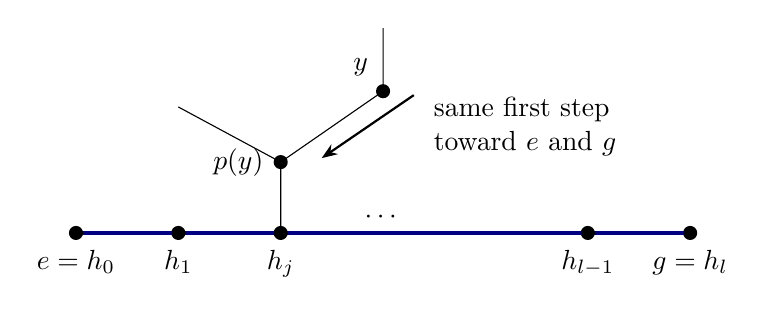
\begin{tikzpicture}[x=1.3cm,y=1cm,vertex/.style={circle,fill=black,inner sep=1.8pt}]
\draw[very thick,blue!50!black] (0,0)--(6,0);
\draw (2,0)--(2,0.9)--(3,1.8)--(3,2.6);
\draw (2,0.9)--(1,1.6);
\draw[-{Stealth[length=2mm]},thick] (3.3,1.75)--(2.4,0.95);
\node[right,align=left] at (3.4,1.35) {same first step\\toward $e$ and $g$};
\node[vertex,label={below:{$e=h_0$}}] at (0,0) {};
\node[vertex,label={below:{$h_1$}}] at (1,0) {};
\node[vertex,label={below:{$h_j$}}] at (2,0) {};
\node at (3,0.2) {$\cdots$};
\node[vertex,label={below:{$h_{l-1}$}}] at (5,0) {};
\node[vertex,label={below:{$g=h_l$}}] at (6,0) {};
\node[vertex,label={left:{$p(y)$}}] at (2,0.9) {};
\node[vertex,label={above left:{$y$}}] at (3,1.8) {};
\end{tikzpicture}
\caption{Off the geodesic $[e,g]$, the first edges toward $e$ and $g$
coincide. Hence $\pi_t(g)\lambda(g)^*$ fixes all basis vectors outside
the finite path span. Only a finite part of the tree is shown.}
\label{fig:tree}
\end{figure}

Let $M_g=\spanop\{\delta_{h_k}:0\le k\le l\}$. On this space define the
truncated shift $S\delta_{h_k}=\delta_{h_{k+1}}$ for $k<l$ and
$S\delta_{h_l}=0$, and put $X\delta_{h_k}=\xi_{h_k}$.
For $R=\operatorname{diag}(1,r,\ldots,r)$, the recursion gives
\begin{equation}\label{eq:X}
X=R(\id-tS^*)^{-1}.
\end{equation}
Indeed, its $k$th column is
$t^k\delta_e+r\sum_{j=1}^k t^{k-j}\delta_{h_j}$.
Since $\norm{S}\le1$ and $\norm{R}=1$,
\begin{equation}\label{eq:Xbound}
\norm{X-\id}\le\norm{R-\id}
+\norm{R}\sum_{j=1}^{\infty}t^j
\le1-r+\frac{t}{1-t}.
\end{equation}
Writing $R'=\operatorname{diag}(r,\ldots,r,1)$,
\eqref{eq:path-action} becomes $T|_{M_g}=XR'-tS$. Therefore
\begin{align*}
\norm{T|_{M_g}-\id}
&\le\norm{(X-\id)R'}+\norm{R'-\id}+t\norm{S}\\
&\le2(1-r)+\frac{t}{1-t}+t=c(t).
\end{align*}
The same bound holds on $K$, since $T$ is the identity on $M_g^\perp$.
Multiplication by $\lambda(g)$ proves \eqref{eq:uniform}. For $g=e$ the
difference is zero, so the supremum includes this case as well.
\end{proof}

\begin{remark}
Only the operator $X$ on a single finite path is used in the estimate.
On this infinitely branching tree, the global map
$\delta_x\mapsto\xi_x$ need not be bounded: the vectors
$\xi_{s_i}$ all have root coefficient $t$. The Gram-matrix construction
of $\pi_t$ does not require such a global bounded map.
\end{remark}

\section{Close inclusions distinguished by a tensor norm}\label{sec:inclusions}

Fix $0<t<1$, let $\pi_t$ be given by Lemma~\ref{lem:tree}, and write
$\pi_0=\lambda$. We construct a common coordinate algebra $D$ and
subalgebras $P_0,P_t$ satisfying Corollary~\ref{cor:obstruction}.
First we record the absorption calculation that will be used both for
closeness and for the tensor-norm estimate.

\begin{lemma}[Absorption]\label{lem:absorption}
Let $\sigma$ be a unitary representation of $G$ on a nonzero Hilbert space
$J$. The operator
\[
W_\sigma(\delta_x\otimes v)=\delta_x\otimes\sigma(x)v
\quad(x\in G,\ v\in J)
\]
is unitary on $K\otimes J$ and satisfies
\begin{equation}\label{eq:absorption}
W_\sigma(\lambda(g)\otimes\id_J)W_\sigma^*
=\lambda(g)\otimes\sigma(g)\quad(g\in G).
\end{equation}
\end{lemma}

\begin{proof}
The operator is the orthogonal direct sum of the unitaries $\sigma(x)$.
On $\delta_x\otimes v$, the left side of \eqref{eq:absorption} equals
\[
\delta_{gx}\otimes\sigma(gx)\sigma(x)^*v
=\delta_{gx}\otimes\sigma(g)v.
\qedhere
\]
\end{proof}

On $L=K\otimes K$, put
\begin{equation}\label{eq:P}
Q_a(g)=\lambda(g)\otimes\pi_a(g),\qquad
P_a=C^*(Q_a(g):g\in G)\quad(a=0,t).
\end{equation}
For the matrix units $E_{xy}\delta_z=\mathbf1_{\{z=y\}}\delta_x$ on $K$,
define $D\subseteq\B(L)$ to be generated by
\begin{equation}\label{eq:D}
\lambda(g)\otimes\id_K,\quad \id_K\otimes\pi_0(g),\quad
\id_K\otimes\pi_t(g)\quad(g\in G),
\qquad \id_K\otimes E_{xy}\quad(x,y\in G).
\end{equation}
The generators include the identity, and $P_0,P_t\subseteq D$.
All three algebras are norm-separable, since their generating sets are
countable.

\begin{lemma}\label{lem:ambient}
The algebra $D$ in \eqref{eq:D} has scalar center, and
\begin{equation}\label{eq:commutant}
D'=\{Y\otimes\id_K:Y\in\lambda(G)'\}.
\end{equation}
There is a unitary $W\in\B(L)$ such that
\begin{equation}\label{eq:close-W}
WP_0W^*=P_t,\qquad \norm{W-\id_L}\le c(t).
\end{equation}
\end{lemma}

\begin{proof}
Commutation with all $\id_K\otimes E_{xy}$ forces a bounded operator to
be $Y\otimes\id_K$: commutation with the diagonal matrix units removes
off-diagonal blocks, and commutation with the remaining units makes the
diagonal blocks identical. The first-factor generators then impose
exactly $Y\in\lambda(G)'$. Such operators commute with all the
second-factor generators, proving \eqref{eq:commutant}. In particular,
$\rho(g)\otimes\id_K\in D'$.

If $Y\otimes\id_K\in Z(D)$, then $Y$ commutes with $\lambda(G)$ by
\eqref{eq:commutant}. It also commutes with $\rho(G)$, since
$Y\otimes\id_K$ belongs to $D$ and the right translations belong to
$D'$. Thus $Y\delta_e$ is invariant under $\lambda(g)\rho(g)$, which
acts on the basis by conjugation $x\mapsto gxg^{-1}$.
Every nonidentity conjugacy class in $G$ is infinite: conjugate a fixed
nonidentity reduced word by distinct generators absent from that word.
A square-summable vector invariant under conjugation must therefore be
supported at $e$. Write $Y\delta_e=\alpha\delta_e$. Commuting with left
translations gives $Y\delta_x=\alpha\delta_x$ for every $x$, proving
$Z(D)=\C\id_L$.

For the final assertion, Lemma~\ref{lem:absorption} shows that
$W=W_{\pi_t}W_{\pi_0}^*$ sends every $Q_0(g)$ to $Q_t(g)$ by conjugation.
Moreover, the direct-sum description of these unitaries gives
\[
\norm{W-\id_L}=\norm{W_{\pi_t}-W_{\pi_0}}
=\sup_{x\in G}\norm{\pi_t(x)-\lambda(x)}\le c(t).
\qedhere
\]
\end{proof}

\begin{lemma}\label{lem:good-inclusion}
The inclusion $P_0\subseteq D$ has the spatial tensor-norm identity.
\end{lemma}

\begin{proof}
Define a unitary on $L$ by
\[
V(v\otimes\delta_x)=\lambda(x)^*v\otimes\delta_x.
\]
It commutes with every element of $D'$ by \eqref{eq:commutant}.
On elementary vectors one computes
\[
VQ_0(g)V^*(v\otimes\delta_x)=v\otimes\delta_{gx}.
\]
Thus $VP_0V^*=\id_K\otimes C^*(\lambda(G))$.
Given finite families $p_i\in P_0$ and $z_i\in D'$, write
\[
Vp_iV^*=\id_K\otimes X_i,\qquad z_i=Y_i\otimes\id_K.
\]
Conjugation by $V$ gives
\[
\norm{\sum_i p_i z_i}=\norm{\sum_i Y_i\otimes X_i}.
\]
On $L\otimes L=K^{\otimes4}$, conjugation by $V\otimes\id_L$ gives
\[
\norm{\sum_i p_i\otimes z_i}
=\norm{\sum_i\id_K\otimes X_i\otimes Y_i\otimes\id_K}
=\norm{\sum_iY_i\otimes X_i}.
\]
The last equality permutes the four tensor factors and uses the fact
that tensoring with a nonzero identity operator does not change norm.
This proves \eqref{eq:tensor-property}.
\end{proof}

For $P_t$, the identity will fail because the product norm has a lower
bound linear in the number of generators, while absorption gives a
square-root upper bound on the tensor norm.

\begin{lemma}\label{lem:free-norm}
For every positive integer $m$,
\begin{equation}\label{eq:free-norm}
\norm{\sum_{i=1}^m\lambda(s_i)}\le2\sqrt m.
\end{equation}
\end{lemma}

\begin{proof}
Let $F_i$ be the orthogonal projection onto the closed span of words beginning
with $s_i^{-1}$. The $F_i$ are pairwise orthogonal. Write
$\lambda(s_i)=A_i+B_i$, where
\[
A_i=\lambda(s_i)(\id_K-F_i),\qquad B_i=\lambda(s_i)F_i.
\]
There is no cancellation when $s_i$ is prepended to a word not beginning
with $s_i^{-1}$. Thus the range of $A_i$ consists of vectors supported on
words beginning with $s_i$, and these ranges are mutually orthogonal.
For every $v\in K$,
\[
\norm{\sum_i A_iv}^2=\sum_i\norm{(\id_K-F_i)v}^2
\le m\norm{v}^2,
\]
while
\[
\norm{\sum_i B_iv}\le\sum_i\norm{F_iv}
\le\sqrt m\left(\sum_i\norm{F_iv}^2\right)^{1/2}
\le\sqrt m\norm{v}.
\]
Adding the two bounds proves \eqref{eq:free-norm}.
\end{proof}

\begin{lemma}\label{lem:bad-inclusion}
For every $0<t<1$, the inclusion $P_t\subseteq D$
fails the spatial tensor-norm identity.
\end{lemma}

\begin{proof}
Choose an integer $m>4/t^2$, so $mt>2\sqrt m$, and take
\[
p_i=Q_t(s_i),\qquad z_i=\rho(s_i)\otimes\id_K,
\qquad 1\le i\le m.
\]
These belong to $P_t$ and $D'$, respectively. Since
$\lambda(s_i)\rho(s_i)\delta_e=\delta_e$, \eqref{eq:coefficient} implies
\begin{equation}\label{eq:large-norm}
\norm{\sum_i p_i z_i}
\ge\left|\inner{\left(\sum_i p_i z_i\right)
(\delta_e\otimes\delta_e)}{\delta_e\otimes\delta_e}\right|
=mt.
\end{equation}
On the other hand, the tensor sum on $L\otimes L$ is
\[
\sum_{i=1}^m\lambda(s_i)\otimes\pi_t(s_i)
\otimes\rho(s_i)\otimes\id_K.
\]
Apply Lemma~\ref{lem:absorption} to the representation
$\sigma=\pi_t\otimes\rho\otimes1$ on $K^{\otimes3}$, where $1$ is the
trivial representation on the last copy of $K$. Together with
Lemma~\ref{lem:free-norm}, it gives
\begin{equation}\label{eq:small-norm}
\norm{\sum_i p_i\otimes z_i}
=\norm{\sum_{i=1}^m\lambda(s_i)}\le2\sqrt m<mt.
\end{equation}
Equations~\eqref{eq:large-norm} and \eqref{eq:small-norm} contradict the
identity for this finite list.
\end{proof}

\section{The counterexamples}\label{sec:assembly}

\begin{proof}[Proof of Theorem~\ref{thm:main}]
Given $\varepsilon>0$, choose $0<t<1$ so small that $2c(t)<\varepsilon$.
Use the algebras $P_0,P_t\subseteq D\subseteq\B(L)$ from
Section~\ref{sec:inclusions}, and put
\[
H=\bigoplus_{n\ge1}L,\qquad A=\E_D(P_0),\qquad B=\E_D(P_t).
\]
The space $H$ is separable. Lemma~\ref{lem:ambient} supplies the scalar
center of $D$, so Proposition~\ref{prop:sequences} shows that $A,B$ are
unital norm-separable $C^*$-algebras with common identity and that
$A''=B''$. The same lemma supplies a unitary $W$ with
$WP_0W^*=P_t$ and $\norm{W-\id_L}\le c(t)$. By
Corollary~\ref{cor:obstruction},
\[
\KK(A,B)\le2c(t)<\varepsilon.
\]
Finally, Lemmas~\ref{lem:good-inclusion} and~\ref{lem:bad-inclusion}
show that the relative tensor-norm identity holds for $P_0$ but not for
$P_t$. Corollary~\ref{cor:obstruction} therefore excludes every unitary
conjugating $A$ onto $B$.
\end{proof}

The common ideal $c_0(\N,D)$ makes the von Neumann closures agree,
while the norm-limit condition retains the distinction between the two
inclusions.

\begin{thebibliography}{99}

\bibitem{BOT13}
M. Burger, N. Ozawa, and A. Thom,
\emph{On Ulam stability},
Israel J. Math. \textbf{193} (2013), 109--129.
\href{https://doi.org/10.1007/s11856-012-0050-z}{doi:10.1007/s11856-012-0050-z}.

\bibitem{CC83}
M.-D. Choi and E. Christensen,
\emph{Completely order isomorphic and close $C^*$-algebras need not be
$*$-isomorphic},
Bull. London Math. Soc. \textbf{15} (1983), no.~6, 604--610.
\href{https://doi.org/10.1112/blms/15.6.604}{doi:10.1112/blms/15.6.604}.

\bibitem{CSSWW10}
E. Christensen, A. M. Sinclair, R. R. Smith, S. A. White, and W. Winter,
\emph{The spatial isomorphism problem for close separable nuclear
$C^*$-algebras},
Proc. Natl. Acad. Sci. USA \textbf{107} (2010), no.~2, 587--591.
\href{https://doi.org/10.1073/pnas.0913281107}{doi:10.1073/pnas.0913281107}.

\bibitem{CSSWW12}
E. Christensen, A. M. Sinclair, R. R. Smith, S. A. White, and W. Winter,
\emph{Perturbations of nuclear $C^*$-algebras},
Acta Math. \textbf{208} (2012), no.~1, 93--150.
\href{https://doi.org/10.1007/s11511-012-0075-5}{doi:10.1007/s11511-012-0075-5}.

\bibitem{Johnson82}
B. E. Johnson,
\emph{A counterexample in the perturbation theory of $C^*$-algebras},
Canad. Math. Bull. \textbf{25} (1982), no.~3, 311--316.
\href{https://doi.org/10.4153/CMB-1982-043-4}{doi:10.4153/CMB-1982-043-4}.

\bibitem{KK72}
R. V. Kadison and D. Kastler,
\emph{Perturbations of von Neumann algebras. I. Stability of type},
Amer. J. Math. \textbf{94} (1972), no.~1, 38--54.
\href{https://doi.org/10.2307/2373592}{doi:10.2307/2373592}.

\bibitem{PS86}
T. Pytlik and R. Szwarc,
\emph{An analytic family of uniformly bounded representations of free groups},
Acta Math. \textbf{157} (1986), 287--309.
\href{https://doi.org/10.1007/BF02392596}{doi:10.1007/BF02392596}.

\end{thebibliography}

\end{document}
